% Template for ICASSP-2021 paper; to be used with:
%          spconf.sty  - ICASSP/ICIP LaTeX style file, and
%          IEEEbib.bst - IEEE bibliography style file.
% --------------------------------------------------------------------------
\documentclass{article}
\usepackage{spconf,amsmath,graphicx}
\usepackage{hyperref}
\hypersetup{
    colorlinks=true,
    linkcolor=[rgb]{0.043,0,0.5},
    citecolor=[rgb]{0.043,0,0.5},
    urlcolor=[rgb]{0.043,0,0.5},
    filecolor=[rgb]{0.043,0,0.5},
    pdftitle={Zafar's website},
}
\usepackage{enumitem}
\usepackage[style=ieee]{biblatex}
\addbibresource{refs.bib}
\usepackage{multimedia}

\title{Ze Awesome French Audio Researcher (ZAFAR)}

\name{Zafar Rafii}
\address{PhD in Electrical Engineering \& Computer Science \\
\texttt{zafarrafii@gmail.com}}

\begin{document}

\maketitle

\begin{abstract}
We present Zafar, Ze Awesome French Audio Researcher. The proposed researcher has a PhD in electrical engineering and computer science from Northwestern University, with a focus on audio signal analysis. He has over 30 publications, including conference papers, journal articles, and patents, with 1,500 citations overall. He is actively involved within the research community, as a reviewer for numerous conferences and journals, a member of the IEEE audio and acoustic signal processing technical committee, and an organizer of networking meetups in the San Francisco Bay Area. He is currently a research engineer manager at Gracenote, where he is working on a number of projects involving, among others, audio recognition, audio separation, and audio classification.
\end{abstract}

\begin{keywords}
Research, audio signal analysis, separation, recognition, classification
\end{keywords}

\section{Introduction}
\label{sec:intro}

% Patents
\nocite{patent_cremer_may2021}
\nocite{patent_rafii_may2021}
\nocite{patent_cremer_feb2021}
\nocite{patent_rafii_jan2021}
\nocite{patent_rafii_dec2020}
\nocite{patent_rafii_oct20202}
\nocite{patent_rafii_oct2020}
\nocite{patent_rafii_jul20202}
\nocite{patent_rafii_jul2020}
\nocite{patent_coover_mar2020}
\nocite{patent_pardo_jul2015}

% Journal Articles
\nocite{article_rafii_nov2018}
\nocite{article_rafii_aug2018}
\nocite{article_rafii_dec2014}
\nocite{article_liutkus_aug2014}
\nocite{article_rafii_jan2013}
\nocite{article_sabin_jun2013}

% Conference Proceedings
\nocite{inproceedings_vartakavi_aug2021}
\nocite{inproceedings_kim_sep2018}
\nocite{inproceedings_seetharaman_mar2017}
\nocite{inproceedings_fitzgerald_mar2017}
\nocite{inproceedings_liutkus_feb2017}
\nocite{inproceedings_ono_aug2015}
\nocite{inproceedings_rafii_apr2015}
\nocite{inproceedings_liutkus_apr2015}
\nocite{inproceedings_fitzgerald_jun2014}
\nocite{inproceedings_liutkus_may2014}
\nocite{inproceedings_rafii_may2014}
\nocite{inproceedings_rafii_nov2013}
\nocite{inproceedings_rafii_may2013}
\nocite{inproceedings_rafii_oct2012}
\nocite{inproceedings_liutkus_mar2012}
\nocite{inproceedings_cartwright_aug2011}
\nocite{inproceedings_rafii_may2011}
\nocite{inproceedings_rafii_may2011_2}
\nocite{inproceedings_rafii_oct2009}

% Chapter Books
\nocite{inbook_pardo_2018}
\nocite{inbook_rafii_2014}

% Technical Reports
\nocite{report_rafii_2009}

% Talks
\nocite{misc_mcdermott_oct2012}

% Data Sets
\nocite{online_rafii_2019}
\nocite{online_rafii_2017}

The proposed researcher is named Zafar Rafii. He received a PhD in electrical engineering and computer science from \href{https://www.northwestern.edu/}{Northwestern University} in 2014. He was with the \href{https://interactiveaudiolab.github.io/}{Interactive Audio Lab} under the supervision of professor Bryan Pardo. Prior to that, he was a research engineer at Audionamix, in France. He is now a research engineer manager in the Applied Research group at \href{https://www.gracenote.com/}{Gracenote}.

\begin{figure}[htb]
\centering
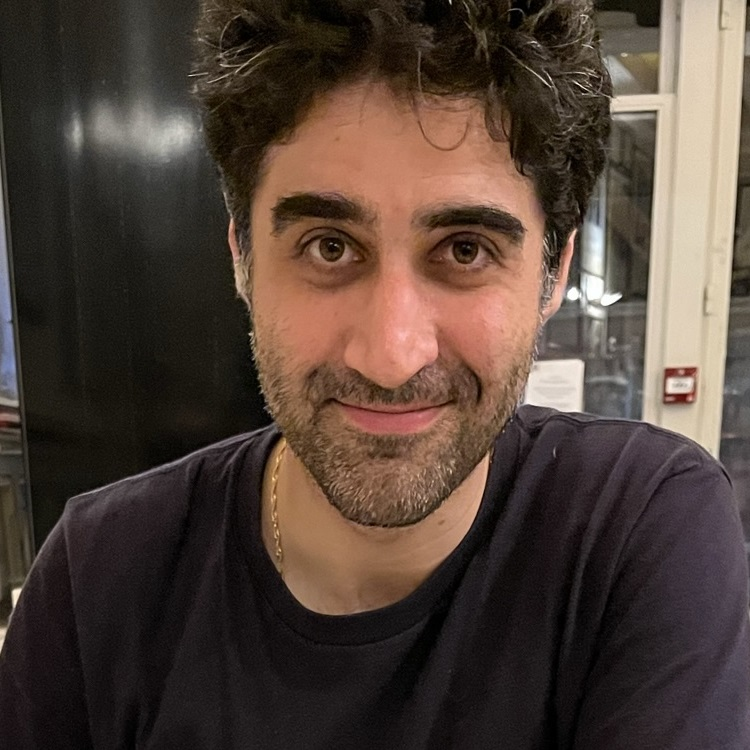
\includegraphics[width=0.5\columnwidth]{Images/zafar.jpg}
\caption{Overview of the proposed researcher.}
\label{fig:zafar}
\end{figure}

The proposed researcher has interest and expertise in audio signal analysis. He has worked on a number of projects, including:
\begin{itemize}[noitemsep,topsep=0pt]
\item Blind source separation
\item Spatial source separation
\item Digital audio effects
\item Audio fingerprinting
\item Cover song identification
\item Audio encoding analysis
\item Audio beamforming
\item Audio watermarking
\item Audio/video segmentation
\item Audio classification
\end{itemize}

For more information on the proposed researcher, the reader is referred to the following materials:
\begin{itemize}[noitemsep,topsep=0pt]
\item \href{http://zafarrafii.com/Zafar Rafii - CV.pdf}{CV}
\item \href{https://github.com/zafarrafii}{GitHub}
\item \href{https://www.linkedin.com/in/zafarrafii/}{LinkedIn}
\item \href{https://scholar.google.com/citations?user=8wbS2EsAAAAJ&hl=en}{Google Scholar}
\end{itemize}

For other relevant information related to the proposed researcher, such as the meetups he organizes, the mentoring program he is involved in, or the audio dataset he created, the reader is referred to the following links:
\begin{itemize}[noitemsep,topsep=0pt]
\item \href{https://www.meetup.com/bishbash/}{SF-BISH Bash meetup}
\item \href{https://www.youtube.com/channel/UCfVTmVY__IObKq06vZFryxA}{SF-BISH Bash YouTube channel}
\item \href{https://wimir.wordpress.com/}{Women in Music Information Retrieval}
\item \href{https://sigsep.github.io/datasets/musdb.html#musdb18-compressed-stems}{MUSDB18 dataset}
\end{itemize}

The rest of the website is organized as follows. In \hyperref[sec:research]{Section 2}, we present a selection of projects the proposed researcher has worked on. In \hyperref[sec:repet]{Section 3}, we introduce his PhD thesis work on the REpeating Pattern Extraction Technique (REPET) for blind source separation. In \hyperref[sec:codes]{Section 4}, we share links to his GitHub repositories where some of his source codes reside. In \hyperref[sec:refs]{Section 5}, we provide references to all of his publications, presentations, and other materials.


\section{Research}
\label{sec:research}

\subsection{Adaptive Reverberation Tool (2008)}
\label{ssec:reverb}

People often think about sound in terms of subjective concepts which do not necessarily have known mappings onto the controls of existing audio tools. For example, a bass player may wish to use a reverberation effect to make her/his bass sound more "boomy", but unfortunately there is no "boomy" knob to be found. We developed a system that can quickly learn an audio concept from a user (e.g., a "boomy" effect) and generate a simple controller than can manipulate sounds in terms of that audio concept (e.g., make a sound more "boomy"), bypassing the bottleneck of technical knowledge of complex interfaces and individual differences in subjective terms.

For this study, we focused on reverberation effects. We developed a digital reverberator, mapping the parameters of the digital filters to measures of the reverberation effect, so that the reverberator can be controlled through meaningful descriptors such as "reverberation time" or "spectral centroid." In the learning process, a sound is first modified by a series of reverberation settings using the reverberator. The user then listens and rates each modified sound as to how well it fits the audio concept she/he has in mind. The ratings are finally mapped onto the controls of the reverberator and a simple controller is built with which the user is able to manipulate the degree of her/his audio concept on a sound. Several experiments conducted on human subjects showed that the system learns quickly (under 3 minutes), predicts user responses well (mean correlation of 0.75), and meets users' expectations (average human rating of 7.4 out of 10).

\begin{figure}[htb]
\centering
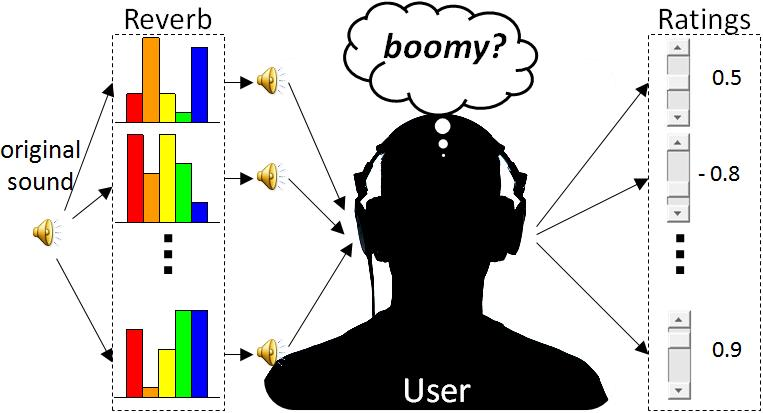
\includegraphics[width=\columnwidth]{Images/reverberation.jpg}
\caption{A listener rating a sound modified by a series of reverberation settings as to how well it fits the audio concept of "boomy" they have in mind.}
\label{fig:reverb}
\end{figure}

For more information about this project, the reader is referred to \cite{article_sabin_jun2013}, \cite{inproceedings_rafii_oct2009}, and 
\cite{report_rafii_2009}.


\subsection{DUET using the CQT (2011)}
\label{ssec:duet}

The Degenerate Unmixing Estimation Technique (DUET) is a blind source separation method that can separate an arbitrary number of unknown sources using a single stereo mixture. DUET builds a two-dimensional histogram from the amplitude ratio and phase difference between channels, where each peak indicates a source, with peak location corresponding to the mixing parameters associated with that source. Provided that the time-frequency bins of the sources do not overlap too much - an assumption generally validated by speech mixtures, DUET partitions the time-frequency representation of the mixture by assigning each bin to the source with the closest mixing parameters. However, when time-frequency bins of the sources start to overlap more - as generally seen in music mixtures when using the common short-time Fourier transform (STFT), peaks start to fuse in the 2d histogram and DUET cannot perform separation effectively.

\begin{figure}[htb]
\centering
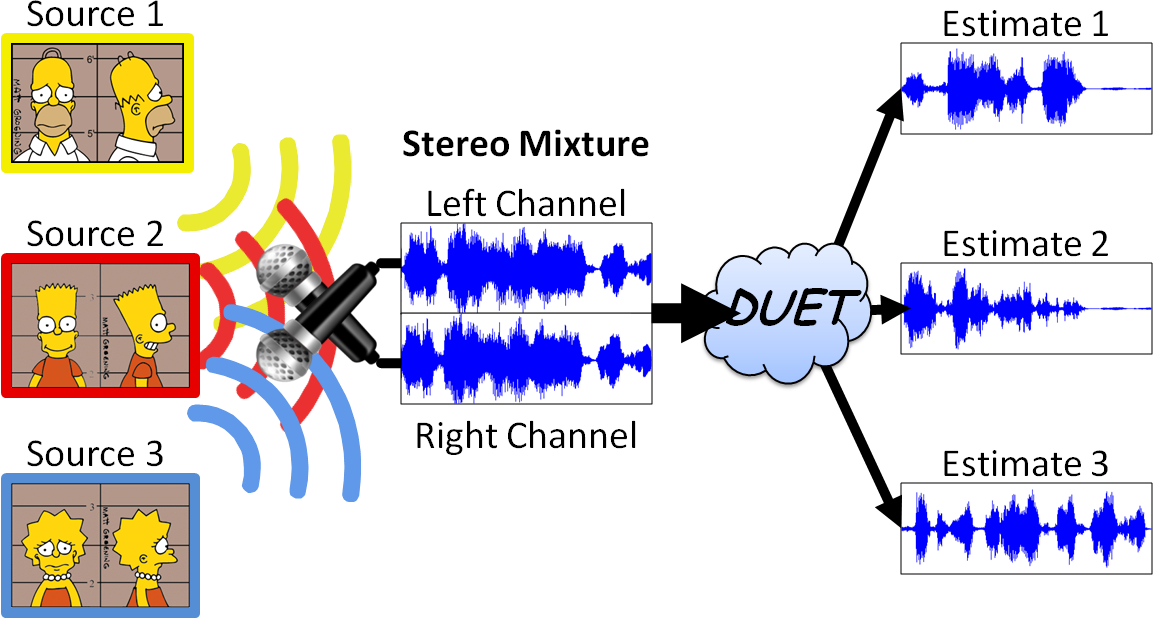
\includegraphics[width=\columnwidth]{Images/duet.png}
\caption{Blind source separation of a stereo recording of Homer, Bart, and Lisa using DUET.}
\label{fig:duet}
\end{figure}

We proposed to improve peak/source separation in DUET by building the 2d histogram from an alternative time-frequency representation based on the constant-Q transform (CQT). Unlike the Fourier transform, the CQT has a logarithmic frequency resolution, mirroring the human auditory system and matching the geometrically spaced frequencies of the Western music scale, therefore better adapted to music mixtures. We also proposed other contributions to enhance DUET, such as adaptive boundaries for the 2d histogram to improve peak resolving when sources are spatially too close to each other, and Wiener filtering to improve source reconstruction. Experiments on mixtures of piano notes and harmonic sources showed that peak/source separation is overall improved, especially at low octaves (under 200 Hz) and for small mixing angles (under ${\pi}/{6}$ rad).

Unlike the classic DUET based on the Fourier transform, DUET combined with the CQT can resolve adjacent pitches in low octaves as well as in high octaves thanks to the log frequency resolution of the CQT:
\begin{itemize}[noitemsep,topsep=0pt]
\item \href{Audio/DUET/piano_mixture.mp3}{Mixture of 3 piano notes}
\item Estimates: \href{Audio/DUET/A2_estimated.mp3}{A2} - \href{Audio/DUET/Bb2_estimated.mp3}{Bb2} -  \href{Audio/DUET/B2_estimated.mp3}{B2}
\item Originals: \href{Audio/DUET/A2_original.mp3}{A2} - \href{Audio/DUET/Bb2_original.mp3}{Bb2} - \href{Audio/DUET/B2_original.mp3}{B2}
\end{itemize}

DUET combined with the CQT and adaptive boundaries helps to improve separation when sources have low pitches (for example, here, between the two cellos) and/or are spatially too close to each other:
\begin{itemize}[noitemsep,topsep=0pt]
\item \href{Audio/DUET/instruments_mixture.mp3}{Mixture of 4 instruments}
\item Estimates: \href{Audio/DUET/cello1_estimated.mp3}{cello 1} - \href{Audio/DUET/cello2_estimated.mp3}{cello 2} - \href{Audio/DUET/flute_estimated.mp3}{flute} - \href{Audio/DUET/strings_estimated.mp3}{strings}
\item Originals: \href{Audio/DUET/cello1_original.mp3}{cello 1} - \href{Audio/DUET/cello2_original.mp3}{cello 2} - \href{Audio/DUET/flute_original.mp3}{flute} - \href{Audio/DUET/strings_original.mp3}{strings}
\end{itemize}

For more information about this project, the reader is referred to \cite{inproceedings_rafii_may2011_2}.


\section{REPET}
\label{sec:repet}


\section{Codes}
\label{sec:codes}


\printbibheading[title={References},heading=bibnumbered]
\label{sec:refs}
\printbibliography[title={Patents},type=patent,heading=subbibnumbered]
\printbibliography[title={Journal Articles},type=article,heading=subbibnumbered]
\printbibliography[title={Conference Proceedings},type=inproceedings,heading=subbibnumbered]
\printbibliography[title={Book Chapters},type=inbook,heading=subbibnumbered]
\printbibliography[title={Technical Reports},type=report,heading=subbibnumbered]
\printbibliography[title={Talks},type=misc,heading=subbibnumbered]
\printbibliography[title={Data Sets},type=online,heading=subbibnumbered]

%\bibliographystyle{IEEEbib}
%\bibliography{refs}

\end{document}
